We now assume that only $b,s,\mu,\tau$ and dark matter particles couple to $Z'$, and dark matter couples exclusively to $Z'$. Taking into account flavour mixing, a tree level interaction of dark matter particles and nucleons is then possible. We take a look at this option in the first section. Afterwards we compare the direct detection cross section of the tree level interaction with the one of the loop interaction presented in \ref{sec:ParamSpace}, respectively \cite{Z}.
\todo{Der Text ist nicht so gut.}

\section{Tree Level Interaction Cross Section}
By considering flavour mixing, a dark matter particle can interact with the strange and bottom parts of a down quark in a nucleus through the tree level diagram shown in figure \ref{fig:Tree}. In terms of the operators in \eqref{eq:chiral}, the diagram corresponds to $Q_{2bs},Q_{2sb}$. The related coefficients are
\begin{align}
	C_{2bs} = C_{2sb}^* = q_\chi\frac{Y_{Qb}Y_{Qs}^*}{2m_Q^2} \ ,
\end{align}
for which \cite{InColour} gives the approximation
\begin{align}\label{eq:BoundC}
\text{Re}\left(C_{2bs}\right) \approx \SI{8e-10}{\giga\electronvolt}^{-2} \ .
\end{align}
This leads to the non-chiral coefficients (see \eqref{eq:CoeffNormal})
\begin{align}
	K_{1,d} &= +\text{Re}(V_{cd}^*V_{td}C_{2sb}) \ , \notag \\
	K_{1,s} &= +\text{Re}(V_{cs}^*V_{ts}C_{2sb}) \ , \notag \\
	K_{3,d} &= -\text{Re}(V_{cd}^*V_{td}C_{2sb}) \ , \notag \\
	K_{3,s} &= -\text{Re}(V_{cs}^*V_{ts}C_{2sb}) \ ,
\end{align}
and all other $K_{l,q}$ vanish. These are the coefficients of the spin-dependent interaction $R_{3,q} = (\bar{\chi}\gamma^\mu\chi)(\bar{q}\gamma_\mu\gamma_5 q)$ and the spin-independent interaction $R_{1,q} = (\bar{\chi}\gamma^\mu\chi)(\bar{q}\gamma_\mu q)$. We neglect the former one because it is various orders of magnitude smaller than the spin-independent cross section. However, there is no interaction with strange quarks as they are only available as sea quarks. Thus, we are left with the spin-independent vector interaction
\begin{align}
	\mathcal{L} = K_{1,d}(\bar{\chi}\gamma^\mu\chi)(\bar{d}\gamma_\mu d) \ .
\end{align}
As explained in \cite[Chapter 7]{Supersymmetric}, this operator counts the number of down quarks. So the nucleon cross section is
\begin{align}\label{eq:Tree}
	\sigma_{0,\text{tree}}^\text{SI} &= \frac{\mu_{A\chi}^2}{A^2\pi}\left|ZC_p +(A-Z)C_n\right|^2 \ ,
\end{align}
where $C_p = K_{1,d}$ and $C_n = 2K_{1,d}$ are the proton and neutron coefficients.


\begin{figure}
	\centering
	\begin{tikzpicture}
\tikzstyle{centerArrow}=[decoration={
markings,
mark=at position 0.5 with {\fill (2pt,0)--(-2pt,2.31pt)--(-2pt,-2.31pt)--cycle;}}]
\begin{scope}[xshift=3cm,yshift=-2cm]
\def\xmove{2}
\def\ymove{1.25}
\def\centerShift{2}
\def\centerSize{0.08cm}
\coordinate (tCenter1) at (0,0);
\coordinate[fill, circle,inner sep=\centerSize] (tCenter2) at (0,-\centerShift cm);
\node (upperLeft) at (-\xmove,\ymove) {$\chi$};
\node (upperRight) at (\xmove,\ymove) {$\chi$};
\node (lowerLeft) at (-\xmove,-\centerShift cm-\ymove cm) {$b_L,s_L$};
\node (lowerRight) at (\xmove,-\centerShift cm-\ymove cm) {$s_L,b_L$};
\node at (0.5,-\centerShift/2) {$Z'$};
\draw [centerArrow,postaction={decorate}]  (upperLeft) -- (tCenter1) ;
\draw [centerArrow,postaction={decorate}]  (tCenter1) -- (upperRight) ;
\draw [centerArrow,postaction={decorate}]  (lowerLeft) -- (tCenter2) ;
\draw [centerArrow,postaction={decorate}]  (tCenter2) -- (lowerRight) ;
\draw [decoration={snake, segment length=1.5mm, amplitude=0.5mm},decorate] (tCenter1) -- (tCenter2) ;
\end{scope}
\end{tikzpicture}
	\caption{Tree level diagram for direct detection considering flavour mixing.}
	\label{fig:Tree}
\end{figure}

\section{Results}
We now compare the nucleon cross sections for the loop interaction $\sigma_{0,\text{loop}}$ (see equation \eqref{eq:Loop} and figure \ref{fig:Loop}) and the tree level interaction $\sigma_{0,\text{tree}}$ (see equation \eqref{eq:Tree} and figure \ref{fig:Tree}). We choose Xenon, which is used in the LUX and XENON100 experiments, as detection material. The most abundant isotope is Xenon-129, therefore $Z = 54, A=129$ \cite{DD}. For the CKM matrix elements we use the values given in \eqref{eq:Wolf}.


In the following we show various plots, in which we follow \cite{Z} with the distinction of the cases $q_\chi= 1$ and $q_\chi=\sfrac{1}{6}$. Remember that for the former the dark matter mass cannot be much larger than $\SI{23}{\giga\electronvolt}$, but for the latter no restriction is made. Therefore we choose different $m_\chi$-axis scales in the plots. The shaded green area always corresponds to $\sigma_{0,\text{loop}}$, whereas the lines visualize $\sigma_{0,\text{tree}}$.


First, we consider the bound \eqref{eq:BoundBS} for $\sigma_{0,\text{loop}}$. Figure \ref{fig:Allgemein} shows $\sigma_{0,\text{loop}}$ (shaded green) within this bound and $\sigma_{0,\text{tree}}$ with various choices for $C_{2bs} = C$ that are in accordance with \eqref{eq:BoundC}. But even for quiet large values of $C_{2bs}$, the tree level cross section cannot reach the loop cross section. This is a strong hint that Altmannshofer et. al. correctly neglected the CKM mixing in their predictions for dark matter direct detection.


Since there are no restrictions concerning the imaginary part of $C_{2bs}$, we enlarged $\text{Im}(C_{2bs})$ until we reached $\sigma_{0,\text{loop}}$ in figure \ref{fig:Im}. But this was only achieved by imaginary parts that are two orders of magnitude larger than the real part of $C_{2bs}$, which we consider unreasonable.
\todo{Warum ist das eigentlich blöd den Imaginärteil so hoch zu machen.}


Second, we concentrate on the relic density condition in \eqref{eq:Relic}. Therefore we set $m_{Z'} = 2m_\chi$ but allow a $\SI{30}{\%}$ tolerance. For $q_\chi=1$, we set $g'$ to the lower bound in \eqref{eq:Boundg}: $g'=\SI{2e-3}{}$, and for $q_\chi=\sfrac{1}{6}$, we guess $g'=\SI{e-2}{}$. Figure \ref{fig:Relic} shows the corresponding loop cross section again as shaded green area. Regarding the tree level cross section we choose $C_{2bs}$ in strong accordance with \eqref{eq:BoundC}. We find that there are regions for $m_\chi$, where the tree level cross section reaches the loop cross section. The shaded lines show the lower bound of these regions. At the lower border of the green area $m_{Z'} = 2m_\chi\cdot 1.3$. The tables \ref{tab:Relic11} and \ref{tab:Relic116} show the obtained lower bounds (l.b.) for the dark matter mass, the resulting values for the $Z'$ mass, and the ratio of the $Z'$ mass and the coupling $g'$. The ratios are clearly far from being within the (approximate) bounds of \eqref{eq:BoundBS} and thus, the region where flavour mixing becomes relevant cannot address the $B\rightarrow K\bar{l}l$ discrepancies.

\begin{table}
\centering
\caption{$q_\chi=1$. Bounds for the dark matter and $Z'$ masses (in \si{\giga\electronvolt}) and ratio $\sfrac{m_{Z'}}{g'}$ (in \si{\giga\electronvolt}).}
\label{tab:Relic11}
\begin{tabular}{l|ccc}
	\toprule
	$C_{2bs}$ in $\si{\giga\electronvolt}^{-2}$ & l. b. for $m_\chi$ & $m_{Z'}$ & $\sfrac{m_{Z'}}{g'}$ \\
	\midrule
	\SI{8e-10}{} & 22 & 57 & \SI{29e3}{} \\
	\SI{8e-10}{}(1+i) & 18 & 48 & \SI{24e3}{} \\
	\SI{3e-9}{} & 11 & 29 & \SI{15e3}{} \\
	\bottomrule
\end{tabular}
\end{table}
\begin{table}
	\centering
	\caption{$q_\chi=\sfrac{1}{6}$. Bounds for the dark matter and $Z'$ masses (in \si{\giga\electronvolt}) and ratio $\sfrac{m_{Z'}}{g'}$ (in \si{\giga\electronvolt}).}
	\label{tab:Relic116}
	\begin{tabular}{l|ccc}
		\toprule
		$C_{2bs}$ in $\si{\giga\electronvolt}^{-2}$ & l. b. for $m_\chi$ & $m_{Z'}$ & $\sfrac{m_{Z'}}{g'}$ \\
		\midrule
		$\sfrac{1}{6}\SI{8e-10}{}$ & 108 & 281 & \SI{28e3}{} \\
		$\sfrac{1}{6}\SI{8e-10}{}$(1+i) & 91 & 237 & \SI{24e3}{} \\
		$\sfrac{1}{6}\SI{3e-9}{}$ & 56 & 146 & \SI{15e3}{} \\
		\bottomrule
	\end{tabular}
\end{table}

\begin{figure}
	\centering
	\begin{subfigure}[]{0.8\textwidth}
		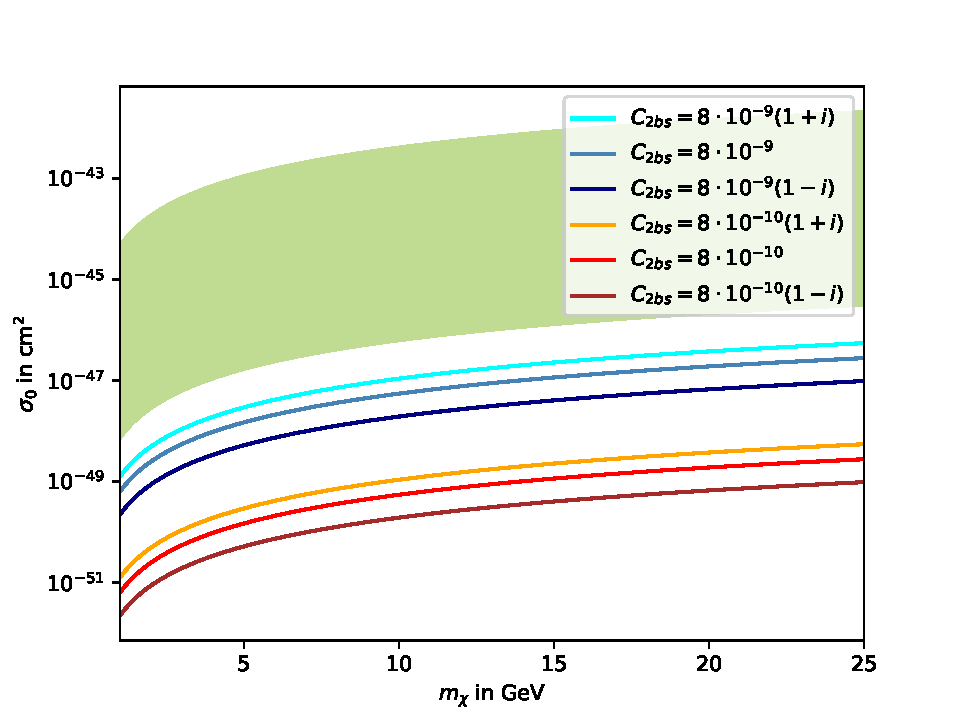
\includegraphics[width=\textwidth]{content/graphics/Allgemein11.pdf}
		\caption{$q_l=q_\chi=1$}
		\label{fig:Allg11}
	\end{subfigure}
	\begin{subfigure}[]{0.8\textwidth}
		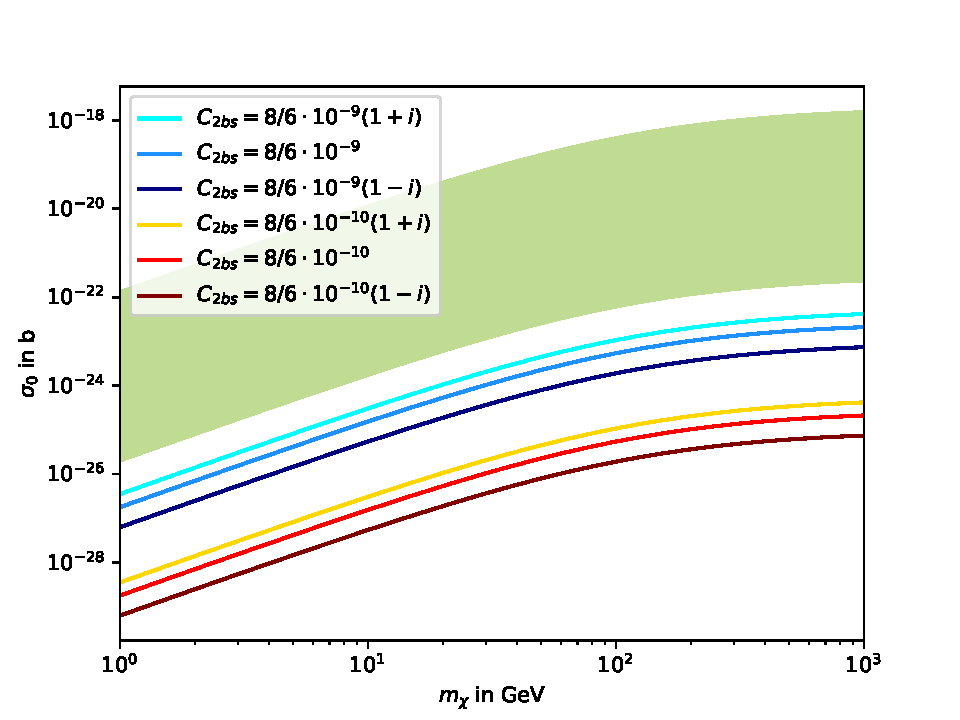
\includegraphics[width=\textwidth]{content/graphics/Allgemein116.pdf}
		\caption{$q_l=1,q_\chi=\sfrac{1}{6}$}
		\label{fig:Allg116}
	\end{subfigure}
	\caption{The shaded green area represents $\sigma_{0,\text{loop}}$ with the bounds in \eqref{eq:BoundBS}. The coloured lines show $\sigma_{0,\text{tree}}$ for different values of $C_{2bs}$ (in $\si{\giga\electronvolt}^{-2}$).}
	\label{fig:Allgemein}
\end{figure}

\begin{figure}
	\centering
	\begin{subfigure}[]{0.8\textwidth}
		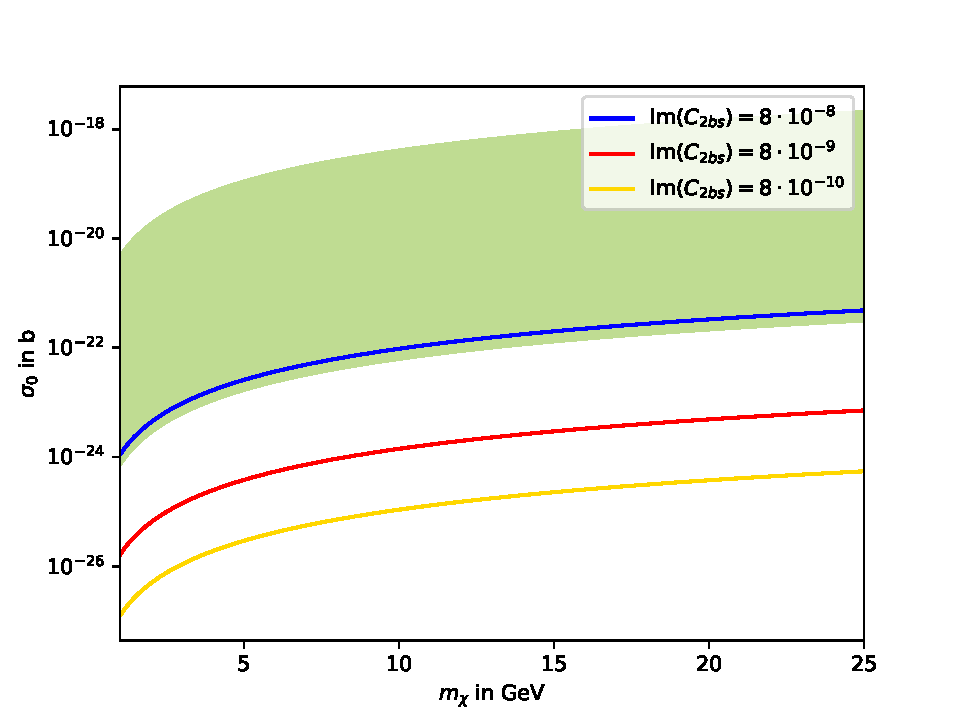
\includegraphics[width=\textwidth]{content/graphics/Im11.pdf}
		\caption{$q_l=q_\chi=1$}
		\label{fig:Im11}
	\end{subfigure}
	\begin{subfigure}[]{0.8\textwidth}
		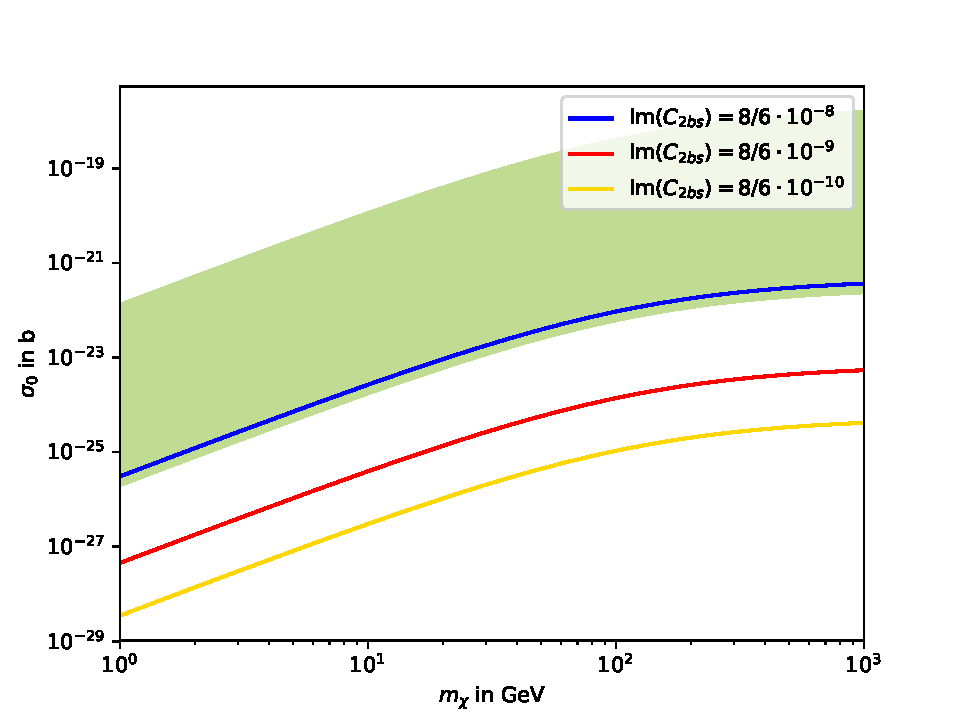
\includegraphics[width=\textwidth]{content/graphics/Im116.pdf}
		\caption{$q_l=1,q_\chi=\sfrac{1}{6}$}
		\label{fig:Im116}
	\end{subfigure}
	\caption{Like \ref{fig:Allgemein}, but the real part of $C_{2bs}$ is fixed at $\SI{8e-10}{\giga\electronvolt}^{-2}$ and only $\text{Im}(C_{2bs})$ is varied.}
	\label{fig:Im}
\end{figure}

\begin{figure}
	\centering
	\begin{subfigure}[]{0.8\textwidth}
		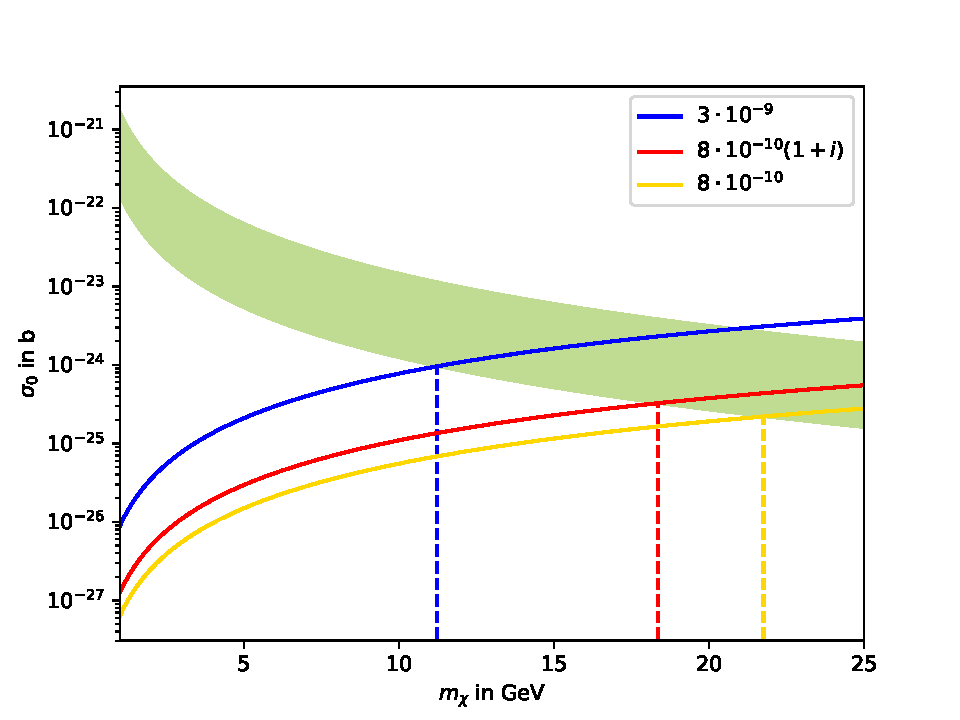
\includegraphics[width=\textwidth]{content/graphics/Relic11.pdf}
		\caption{$q_l=q_\chi=1,g'=\SI{2e-3}{}$}
		\label{fig:Relic11}
	\end{subfigure}
	\begin{subfigure}[]{0.8\textwidth}
		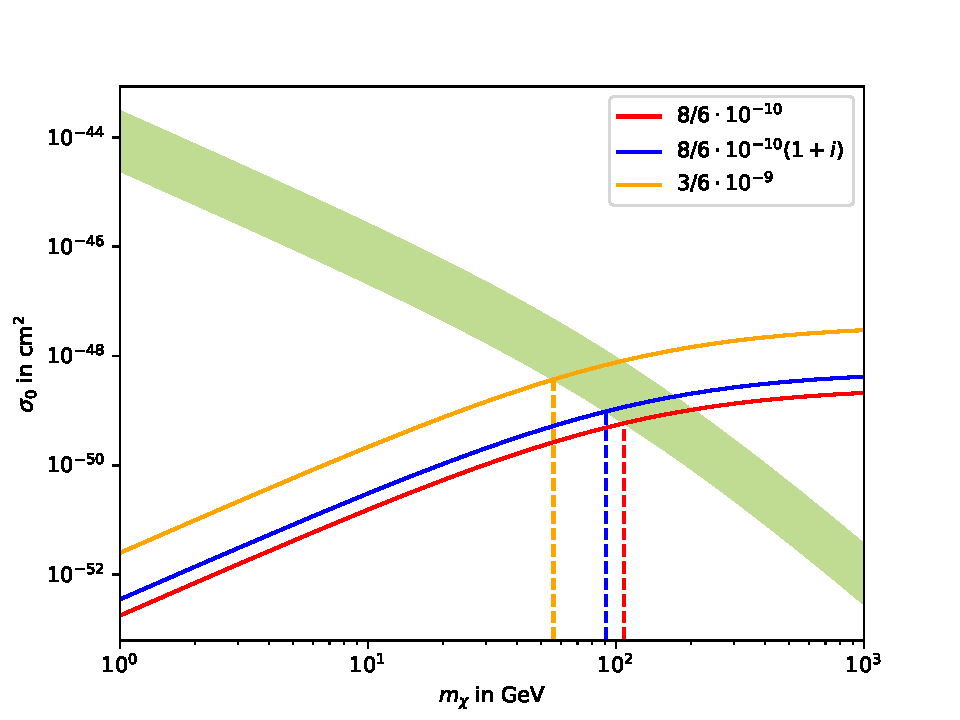
\includegraphics[width=\textwidth]{content/graphics/Relic116.pdf}
		\caption{$q_l=1,q_\chi=\sfrac{1}{6},g'=\SI{e-2}{}$}
		\label{fig:Relic116}
	\end{subfigure}
	\caption{The shaded green area represents the loop cross section $\sigma_{0,\text{loop}}$ at fixed coupling constant $g'$ and $m_{Z'} = 2m_\chi$ with a $\pm\SI{30}{\%}$ tolerance.}
	\label{fig:Relic}
\end{figure}


To make a long story short, if we respect the given bounds from the $B\rightarrow K\bar{l}l$ anomalies, we cannot find any parameter configuration for which the flavour mixing becomes relevant. So, Altmannshofer et. al. correctly neglect quark flavour mixing in the nucleus. However, the set-up presented in chapter \ref{sec:formalism} is universal and may, for example, be applied in the future to check whether ignoring flavour mixing was right in other new physics propositions.